\chapter{Introducción}
\label{cap:capitulo1}
\setcounter{page}{1}

\begin{flushright}
\begin{minipage}[]{7cm}
\emph{La tecnología solo es útil si se pone al servicio de las personas.}\\
\end{minipage}\\

Tim Berners-Lee\\
\end{flushright}

\vspace{0.5cm}

Desde hace varias décadas, la forma en la que las personas interactúan con su entorno en el día a día se ha visto transformada por los numerosos avances de la tecnología. Siguiendo esta dinámica, el campo de la robótica, que estaba limitada en sus inicios al ámbito industrial, se está convirtiendo ahora en una herramienta muy presente en muchos aspectos de la vida cotidiana.La integración de sistemas automatizados fuera de la industria ha dado pie a nuevas aplicaciones, principalmente en el ámbito sanitario y del hogar, consiguiendo mejorar la calidad de vida, la eficiencia en tareas diarias o la autonomía personal.

\

\section{La robótica}
\label{sec:miseccion} % etiqueta para luego referenciar esta sección

La robótica es una disciplina de la ingeniería que se dedica al estudio, diseño, construcción y programación de sistemas capaces de realizar tareas de manera autónoma o semi-autónoma. La robótica es un campo interdisciplinar en el que intervienen áreas como la electrónica, la mecánica, la informática o la inteligencia artificial. Su origen viene de la necesidad de automatizar tareas, reducir el esfuerzo físico que estas requieren y aumentar la precisión en determinados procesos. A pesar de que el término \textit{robot} es relativamente reciente, el concepto de desarrollar máquinas capaces de realizar acciones de manera autónoma ha estado presente desde la antigüedad, donde se diseñaron los primeros autómatas mecánicos con objetivos de investigación experimental, entretenimiento o demostrativos.\\

\
\

La robótica, como rama de la tecnología, comenzó a consolidarse a mediados del siglo XX como resultado del proceso de industrialización iniciado con la Revolución Industrial y, particularmente, al crecimiento de la producción en cadena como se muestra en la Figura~\ref{fig:evolucion_industria}. En este contexto aparecieron los sistemas automatizados iniciales con la capacidad de realizar movimientos repetitivos con una precisión elevada. Estos robots iniciales fueron creados para funcionar en ambientes muy estructurados, donde las condiciones laborales eran conocidas y estaban controladas, lo que hacía posible una programación rígida y predecible en los robots. Se utilizaban sobre todo en el sector industrial para funciones como soldadura, ensamblaje o manipulación de materiales pesados.\\

\begin{figure}[H]
  \centering
  \begin{minipage}[t]{0.45\textwidth}
    \centering
    \includegraphics[height=5cm,width=7.5cm]{figs/Unimate-cadena-montaje.jpg}

    \small a) General Motors introduce Ultimate robots de soldadura por puntos.
  \end{minipage}
  \hfill
  \begin{minipage}[t]{0.45\textwidth}
    \centering
    \includegraphics[height=5cm,width=7.5cm]{figs/Fanuc_cadena_montaje.jpg}

    \small b) Cadena de montaje actual en la industria automovilística.
  \end{minipage}

  \caption{Evolución de la producción en cadena de automóviles con brazos robóticos.}
  \label{fig:evolucion_industria}
\end{figure}

\

La robótica industrial representó un progreso relevante en cuanto a seguridad y productividad. Al delegar a sistemas automáticos aquellas actividades que son repetitivas, peligrosas o que demandan una alta exigencia física, se logró disminuir la cantidad de errores cometidos por humanos y reducir al mínimo los riesgos de accidentes en el trabajo. En esta fase, el avance de la robótica estuvo muy influido por el progreso de la mecánica, la electrónica y los sistemas de control. Estos avances hicieron posible que se aumentara la fiabilidad, velocidad y exactitud de los robots al realizar las tareas. No obstante, estos sistemas continuaban estando limitados a entornos cerrados y claramente definidos, donde la interacción con los humanos era casi nula.\\

\

\

Compañías especializadas en el sector de la robótica industrial han guiado históricamente el desarrollo y la implementación de estos sistemas, marcando así el progreso del sector. Se destacan entre ellas empresas como KUKA\footnote{\url{https://www.kuka.com/es-es}} y ABB\footnote{\url{https://new.abb.com/es}}, que son reconocidas a nivel mundial por la creación y diseño de brazos robóticos industriales, los cuales se usan con frecuencia en las líneas de producción automatizadas. En la Figura~\ref{fig:robots_abb} se muestran algunos robots industriales desarrollados por ABB.\\

\begin{figure} [H]
  \begin{center}
    \includegraphics[height=4.5cm,width=7.5cm]{figs/ABB_FlexPicker.jpg}
    \includegraphics[height=4.5cm,width=7.5cm]{figs/abb_brazo}
  \end{center}
  \caption{Algunos de los robots industriales de la compañía ABB.}
  \label{fig:robots_abb}
\end{figure}

Estas compañías han colaborado de manera crucial en la estandarización, fiabilidad y crecimiento de este tipo de robótica en áreas como la manufactura, la electrónica y la automoción. En la Figura~\ref{fig:evolucion_kuka} se puede ver la evolución en los robots de KUKA y las transformaciones significativas desde sus primeras versiones hasta sus últimos modelos.\\

\begin{figure}[H]
  \centering
  \begin{minipage}[t]{0.45\textwidth}
    \centering
    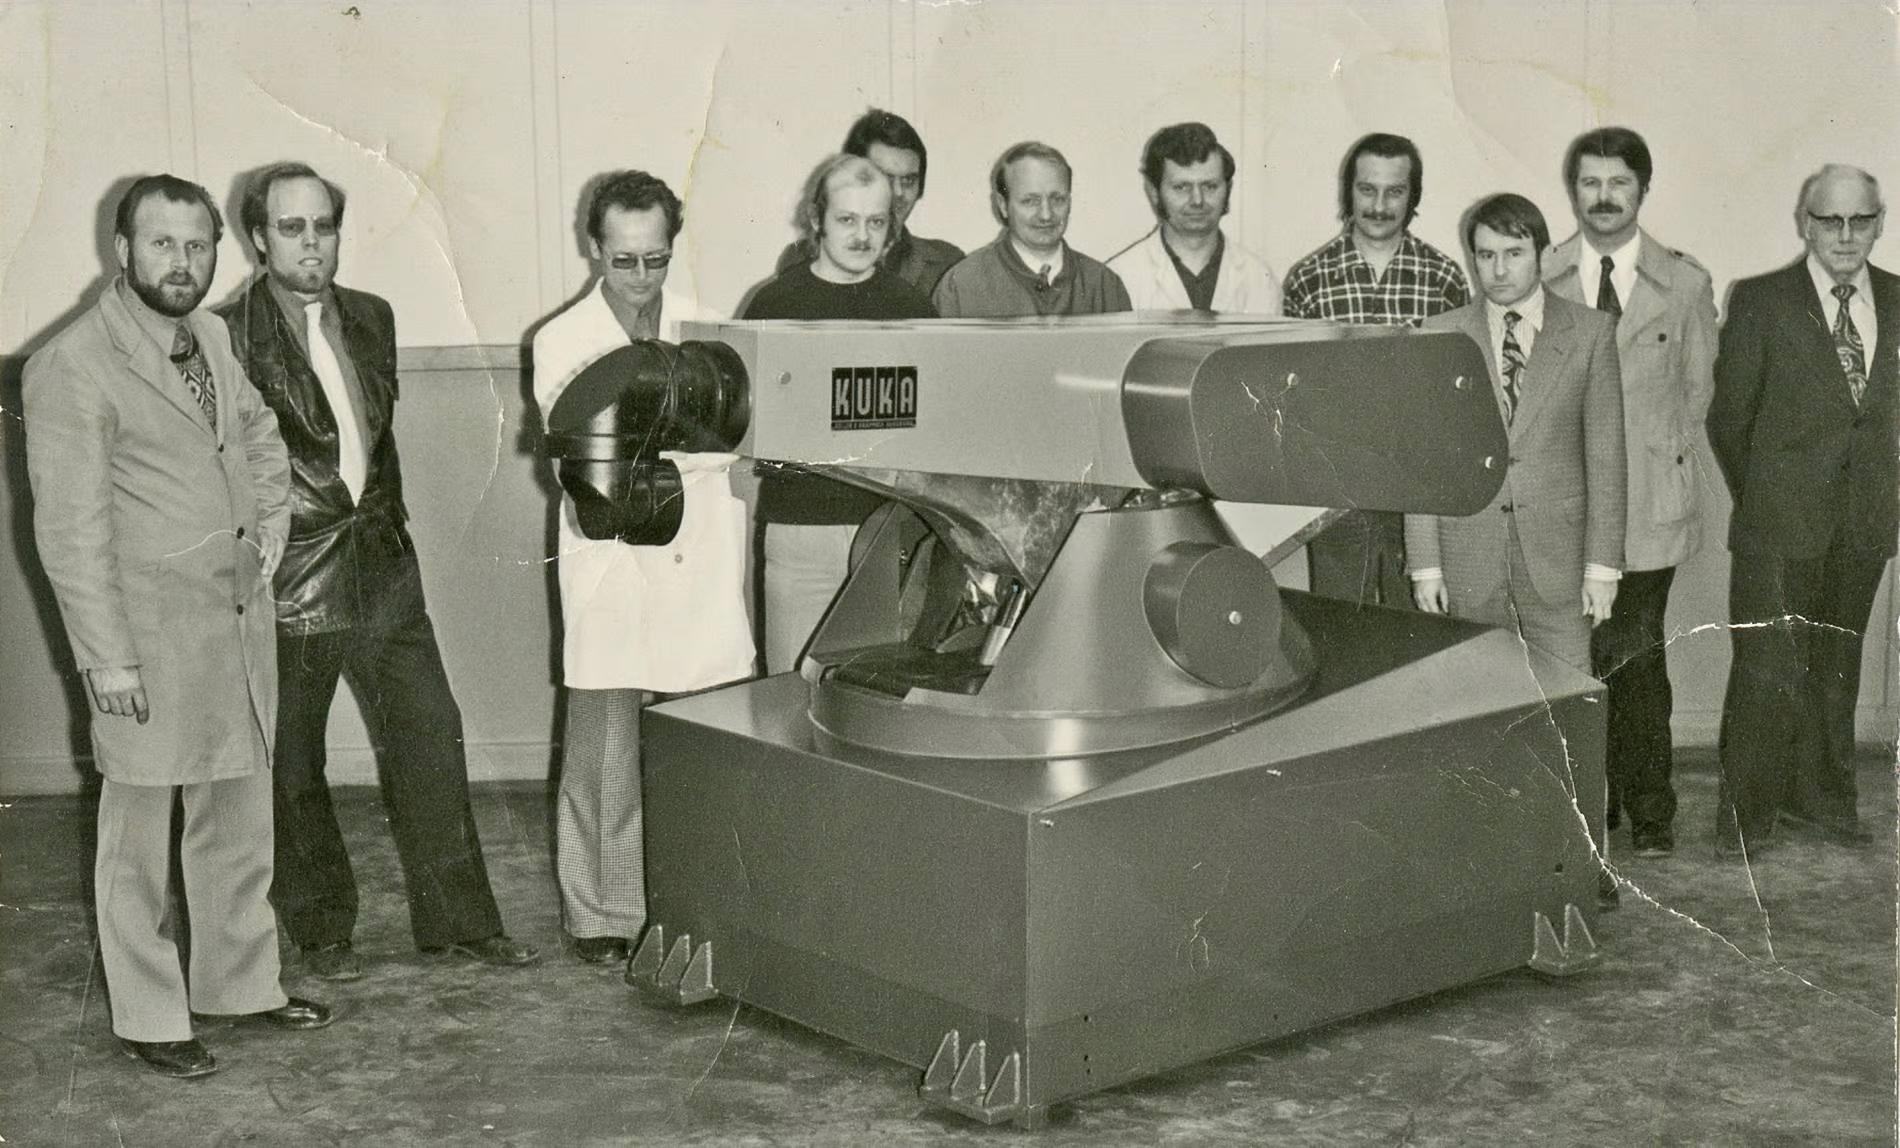
\includegraphics[height=4.5cm,width=7.5cm]{figs/primer_robot_industrial.png}

    \small a) Primer robot industrial con motor eléctrico diseñado por KUKA.
  \end{minipage}
  \hfill
  \begin{minipage}[t]{0.45\textwidth}
    \centering
    \includegraphics[height=4.5cm,width=7.5cm]{figs/brazo_kuka.png}

    \small b) Brazo robótico industrial de KUKA en la actualidad.
  \end{minipage}

  \caption{Evolución de los robots industriales de KUKA.}
  \label{fig:evolucion_kuka}
\end{figure}

\
\

Debido al importante desarrollo ligado a la inclusión de nuevas herramientas y componentes, sobre todo en las últimas décadas del siglo XX, la robótica ha experimentado una evolución significativa. Gracias a la optimización de componentes como los sensores, los robots fueron capaces de recolectar información del entorno, y la evolución en computación y electrónica posibilitó el procesamiento de grandes volúmenes de datos en tiempo real. Además, la creación de sistemas de control más avanzados permitió que los robots tuvieran una mayor habilidad para adaptarse a los cambios en su entorno de trabajo.\\

Esta evolución propició un cambio gradual de sistemas totalmente automatizados a sistemas robóticos con una autonomía más elevada. Los robots dejaron de ser máquinas que ejecutaban secuencias de movimientos predeterminados y empezaron a incorporar procesos para tomar decisiones basados en información del entorno. Así, la robótica de hoy en día se concentra en crear sistemas más versátiles que puedan reaccionar frente a circunstancias imprevistas y desenvolverse en contextos cambiantes como los de la Figura~\ref{fig:ejemplos_colab}.\\

\begin{figure}[H]
  \centering
  \begin{minipage}[t]{0.45\textwidth}
    \centering
    \includegraphics[height=5cm,width=7.25cm]{figs/amazon_warehouse.png}

    \small a) Robots del Amazon Warehouse automatizados para logística.
  \end{minipage}
  \hfill
  \begin{minipage}[t]{0.45\textwidth}
    \centering
    \includegraphics[height=5cm,width=7.25cm]{figs/Cobot.png}

    \small b) Robot colaborativo (cobot) en operación conjunta con un operario.
  \end{minipage}

  \caption{Ejemplos de robots versátiles en entornos cambiantes.}
  \label{fig:ejemplos_colab}
\end{figure}

Hoy en día, la robótica se fundamenta cada vez más en métodos sofisticados de inteligencia artificial para otorgar a los sistemas robóticos habilidades superiores de percepción, razonamiento y toma de decisiones. Estas técnicas posibilitan el procesamiento de cantidades enormes de datos provenientes de sensores y la realización de acciones autónomas, sobrepasando así las restricciones que presentan los sistemas tradicionales de control, que se basan solo en modelos rígidos o reglas inamovibles.\\

\

En este entorno, los enfoques de aprendizaje automático, especialmente el aprendizaje profundo \textit{deep learning}, han desempeñado un papel esencial en la evolución de la robótica moderna. Estas perspectivas posibilitan que los sistemas se instruyan con datos, optimicen su comportamiento conforme ganan experiencia y enfrenten problemas complejos que son difíciles de modelar explícitamente. En la Figura~\ref{fig:ejemplos_tr} vemos cómo los robots planifican trayectorias independientemente de la dificultad de la superficie.\\

\begin{figure} [H]
  \begin{center}
    \includegraphics[height=4.5cm,width=9cm]{figs/planificacion_trayectorias.png}
  \end{center}
  \caption{Ejemplo de planificación de trayectorias.}
  \label{fig:ejemplos_tr}
\end{figure}

Históricamente la visión artificial ha sido uno de los sensores más importantes en los sistemas robóticos, sobre todo en aplicaciones de manipulación, inspección y guiado. Sin embargo, por décadas su rendimiento estuvo restringido debido a las limitaciones en el procesamiento, lo que ocasionaba un embotellamiento computacional al lidiar con la alta cantidad de datos generados por sensores ópticos y cámaras. En la Figura~\ref{fig:ejemplos_dl} vemos cómo los robots son capaces de detectar patrones y clasificar objetos.

\begin{figure} [H]
  \begin{center}
    \includegraphics[height=7.25cm,width=15cm]{figs/deep_learning.jpg}
  \end{center}
  \caption{Ejemplo de clasificación de objetos.}
  \label{fig:ejemplos_dl}
\end{figure}

En los últimos años, la fusión de métodos avanzados de inteligencia artificial, especialmente aquellos que se apoyan en el aprendizaje profundo, con el aumento notorio de la capacidad de cálculo, ha permitido superar estas limitaciones. En consecuencia, los sistemas robóticos actuales son capaces de procesar información visual en tiempo real con más exactitud, rapidez y robustez. Esto ha mejorado significativamente su autonomía y su habilidad para adaptarse a entornos no controlados. Una estructura básica de los sistemas basados en visión se puede ver en la Figura~\ref{fig:ia_diagram}\\

\begin{figure} [H]
  \begin{center}
    \includegraphics[width=0.9\textwidth]{figs/ia_diagram.png}
  \end{center}
  \caption{Arquitectura conceptual de un sistema robótico moderno basado en percepción y toma de decisiones (imagen generada por IA).}
  \label{fig:ia_diagram}
\end{figure}

La robótica, a raíz de estos avances en capacidad de procesamiento, percepción y aprendizaje profundo, ha empezado a sobrepasar los espacios industriales muy estructurados para ir incorporándose poco a poco a áreas que comparte con seres humanos. Los entornos humanos son dinámicos, parcialmente observables y difíciles de modelar con determinismo, en contraste con las líneas de producción convencionales.\\

Los robots son capaces de identificar cambios en el ambiente, prever riesgos potenciales y analizar con más exactitud las acciones humanas gracias a los avances en los sistemas visuales y en los algoritmos de aprendizaje profundo. Además, la capacidad de cálculo aumentada permite la planificación de trayectorias y la toma de decisiones en tiempo real, lo que es esencial para asegurar que la interacción sea fluida y segura.\\

En la Figura~\ref{fig:ejemplos_hr} vemos casos donde hay interacción humano-robot en entornos públicos como el supermercado o la calle.\\

\begin{figure} [H]
  \begin{center}
    \includegraphics[height=5cm,width=7.5cm]{figs/robot_supermercado.png}
    \includegraphics[height=5cm,width=7.5cm]{figs/serve-robot.jpeg}
  \end{center}
  \caption{Ejemplos de robots colaborativos con interacción humano-robot.}
  \label{fig:ejemplos_hr}
\end{figure}

\

En conjunto, estos progresos han hecho posible la creación de sistemas que pueden trabajar con seres humanos de forma adaptativa y segura, lo cual ha promovido nuevas líneas de investigación en seguridad funcional, diseño de robots asistenciales fuera del entorno puramente industrial e interacción humano-robot. El surgimiento de una nueva rama enfocada en crear este tipo de sistemas, ha sido favorecido por este proceso de transformación tecnológica. La robótica de servicio es el campo que surge a raíz de esta necesidad. Esta incluye sistemas creados para la ayuda en la ejecución de tareas cotidianas o profesionales mediante la interacción directa entre las personas y los robots, lo que se discutirá con más profundidad en la Sección~\ref{sec:segundaseccion}.

\

\section{Robótica de servicio}
\label{sec:segundaseccion}

La robótica de servicio abarca a todos los sistemas robóticos que han sido diseñados para ser un servicio accesible para las personas, ya sea en entornos profesionales como en el ámbito personal, siempre fuera del contexto industrial. Lo que la diferencia de la robótica industrial es que opera en entornos menos controlados y estructurados y, además, tiene una interacción cercana con los usuarios. Esto presenta desafíos adicionales con respecto al diseño, la interacción y el control, a diferencia de la robótica industrial, que trabaja en escenarios muy estructurados y controlados.\\

\

La robótica de servicio se divide generalmente en dos grandes categorías: robots de servicio profesionales y robots de servicio personales. Los robots profesionales están destinados a entornos laborales específicos y son operados por personal cualificado, como ocurre en el caso de los robots médicos quirúrgicos, los robots logísticos utilizados en almacenes, los sistemas de inspección industrial o los robots de seguridad y vigilancia. En la Figura~\ref{fig:ejemplos_rspro} vemos dos ejemplos profesionales.

\begin{figure}[H]
  \centering
  \begin{minipage}[t]{0.45\textwidth}
    \centering
    \includegraphics[height=4.75cm,width=7.25cm]{figs/Da-Vinci_01-1.jpg}

    \small a) Robot quirúrgico DaVinci de Intuitive Surgical.
  \end{minipage}
  \hfill
  \begin{minipage}[t]{0.45\textwidth}
    \centering
    \includegraphics[height=4.75cm,width=7.25cm]{figs/logistico.jpg}

    \small b) Robot logístico en almacén de Mobile Industrial Robots (MiR).
  \end{minipage}

  \caption{Ejemplos de robots de servicio en entornos profesionales.}
  \label{fig:ejemplos_rspro}
\end{figure}

Por otro lado, los robots de servicio personales están diseñados para ser utilizados directamente por usuarios no especializados en entornos cotidianos. Dentro de esta categoría se incluyen los robots domésticos de limpieza, los robots asistenciales orientados al apoyo de personas mayores o con discapacidad, los robots educativos y de entretenimiento, así como los asistentes virtuales integrados en dispositivos inteligentes del hogar. En la Figura~\ref{fig:ejemplos_rsp} vemos diferentes tipos de robots de servicio personales.\\

\begin{figure}[H]
  \centering
  \begin{minipage}[t]{0.45\textwidth}
    \centering
    \includegraphics[height=6.25cm,width=6.5cm]{figs/bestic.png}

    \small a) Bestic de Bestic AB: robot de asistencia para comer.
  \end{minipage}
  \hfill
  \begin{minipage}[t]{0.45\textwidth}
    \centering
    \includegraphics[height=6.25cm,width=6.5cm]{figs/ecovast.jpg}

    \small b) Robot limpia cristales Wimbot de Ecovast.
  \end{minipage}

  \caption{Ejemplos de la robótica de servicio en aplicaciones personales.}
  \label{fig:ejemplos_rsp}
\end{figure}

Una de las cualidades esenciales de la robótica de servicio es que requiere una interacción íntima, segura y natural con los seres humanos. Estos sistemas están orientados a usuarios que, en general, no poseen conocimientos técnicos especializados, por lo que deben ser fiables, seguros y fáciles de utilizar. En estas circunstancias es fundamental el diseño de interfaces accesibles e intuitivas, además del ajuste del comportamiento del robot al usuario, para asegurar una experiencia de uso óptima.\\

Un subcampo de la robótica de servicio que se destaca es la robótica doméstica. Este tipo de robótica está enfocada en funcionar dentro del hogar y busca simplificar la ejecución de tareas diarias, optimizar la autonomía personal y ofrecer comodidad y protección a los usuarios. El entorno doméstico representa retos adicionales en comparación con otros contextos de aplicación, ya que tiene una naturaleza no estructurada y presenta una amplia variedad de situaciones. Esto requiere sistemas que sean flexibles, adaptables y tengan la capacidad de desenvolverse en diferentes escenarios. La Figura~\ref{fig:ejemplos_rs} ilustra ejemplos típicos de este tipo de sistemas que son comunes en el entorno doméstico.

\begin{figure}[H]
\centering

\subfigure[Robot aspirador Roomba de iRobot.]{
    \includegraphics[height=4.75cm, width=0.3\textwidth]{figs/iRobot.jpg}
}
\hfill
\subfigure[Pantalla inteligente con Alexa.]{
    \includegraphics[height=4.75cm, width=0.3\textwidth]{figs/echo_show.jpg}
}
\hfill
\subfigure[Robot cortacésped autónomo de Stiga.]{
    \includegraphics[height=4.75cm, width=0.3\textwidth]{figs/stiga.jpg}
}

\caption{Ejemplos de robots de servicio en el ámbito doméstico.}
\label{fig:ejemplos_rs}
\end{figure}

La robótica de servicio, y específicamente la robótica doméstica, ha tenido un crecimiento significativo en los años recientes. El desarrollo de nuevos dispositivos que buscan mejorar la calidad de vida de las personas ha sido motivado por elementos como el envejecimiento paulatino de la población, el aumento en la demanda de soluciones personalizadas y los avances en tecnologías, incluyendo las comunicaciones, los sistemas embebidos y la inteligencia artificial. Este entorno ha propiciado que surjan soluciones cada vez más asequibles y accesibles, lo cual ha fortalecido la robótica de servicio como uno de los sectores con el mayor interés en la robótica contemporánea.

Las aplicaciones de la robótica de servicio que se centran en ayudar a las personas en su vida cotidiana, como los robots asistenciales, son algunas de las más significativas. Estos sistemas tienen como objetivo brindar asistencia en tareas fundamentales, proporcionar acompañamiento o hacer más accesibles ciertas actividades, sobre todo a grupos de personas con necesidades especiales o de la tercera edad. Un ejemplo de robot asistencial que está diseñado para ayudar a personas mayores en el hogar se muestra en la Figura~\ref{fig:robot_asistencial}.\\


\begin{figure} [H]
  \begin{center}
    \includegraphics[width=10cm]{figs/robot_asistencial.jpg}
  \end{center}
  \caption{Robot asistencial para personas mayores.}
  \label{fig:robot_asistencial}
\end{figure}

La importancia de la robótica de servicio en aplicaciones relacionadas con el bienestar y la salud ha quedado demostrada por su integración gradual en áreas asociadas al cuidado personal y a la asistencia a los usuarios. En este marco, la robótica aplicada a la asistencia sanitaria se presenta como una extensión lógica de la robótica de servicio, diseñada para enriquecer la atención médica y ayudar en las tareas vinculadas con el seguimiento, el cuidado y la ayuda a personas, ya sea en clínicas o en la propia casa. En la Sección~\ref{sec:subseccion} veremos de que trata la robótica sanitaria.


%Ni tampoco olvides de poner las URLs como notas al pie. Por ejemplo, si hablo de la Robocup\footnote{\url{http://www.robocup.org}}.
\
\section{Robótica aplicada a la asistencia sanitaria}
\label{sec:subseccion}

La robótica en el sector de la salud es un campo firme dentro de la robótica de servicio. La cirugía asistida por robot, en particular los procedimientos mínimamente invasivos, ha mostrado su viabilidad clínica desde hace más de veinte años gracias a sistemas como el \textit{Da Vinci Surgical System} o el \textit{ROSA} que se muestra en la Figura~\ref{fig:rosa}.

\begin{figure} [H]
  \begin{center}
    \includegraphics[height=9.5cm, width=\textwidth]{figs/rosa.jpg}
  \end{center}
  \caption{ROSA Sistema robótico de apoyo en neurocirugía.}
  \label{fig:rosa}
\end{figure}

Tradicionalmente, estas tecnologías han sido creadas en hospitales, enfocadas en la cirugía, el apoyo al personal de salud y la rehabilitación. Hoy en día, el campo se ha extendido a nuevas áreas tales como la logística de los hospitales, la asistencia no invasiva y el seguimiento constante del paciente. La Figura~\ref{fig:robotica_sanitaria} muestra ejemplos de estas aplicaciones en diversas situaciones clínicas.

\begin{figure}[H]
\centering
\subfigure[\centering Robot autónomo Moxi para logística hospitalaria.]{
    \includegraphics[height=7.25cm, width=7.25cm]{figs/robot_hospital.jpg}
}
\hfill
\subfigure[\centering Sistema robótico de asistencia o rehabilitación.]{
    \includegraphics[height=7.25cm, width=7.25cm]{figs/rehab.jpeg}
}

\caption{Aplicaciones representativas de la robótica sanitaria.}
\label{fig:robotica_sanitaria}
\end{figure}

La robótica asistencial aplicada a la salud, cuyo propósito esencial es ayudar a las personas en tareas vinculadas con su bienestar físico y su cuidado cotidiano, aparece en este escenario. Estos sistemas no tienen el objetivo de reemplazar al personal médico, sino que buscan ser una herramienta adicional para disminuir errores, incrementar la seguridad y optimizar la autonomía de los usuarios. Además, la implementación de soluciones robóticas en el sector sanitario ayuda a mejorar los recursos existentes y a proporcionar una atención más individualizada.\\

\begin{figure} [H]
  \begin{center}
    \includegraphics[width=\textwidth]{figs/CMR-Versius.png}
  \end{center}
  \caption{Sistema quirúrgico Versius para cirugía mínimamente invasiva.}
  \label{fig:versius}
\end{figure}

El Versius Surgical System, creado por CMR Surgical\footnote{\url{https://cmrsurgical.com/}}, es un sistema quirúrgico que destaca en los avances actuales de la robótica sanitaria. Como se ve en la Figura~\ref{fig:versius}, está diseñado para realizar cirugías mínimamente invasivas y tiene una estructura modular. El sistema TUG de Aethon\footnote{\url{https://aethon.com/}} se utiliza para trasladar de manera autónoma ropa hospitalaria, material clínico y medicinas en los hospitales, dentro del área de automatización sanitaria. En cuanto a la rehabilitación neuromotora, el sistema Lokomat, creado por Hocoma\footnote{\url{https://www.hocoma.com/us/solutions/lokomat/}}, posibilita que la terapia asistida de la marcha se realice a través de un exoesqueleto robótico que controla el movimiento por medio de una computadora y soporta el peso corporal. Se pueden ver estas soluciones tecnológicas para logística y terapia asistida en la Figura~\ref{fig:ejemplos_reales_hp}.\\

\

\

\begin{figure}[H]
  \centering
  \begin{minipage}[t]{0.45\textwidth}
    \centering
    \includegraphics[height=7.5cm,width=7.75cm]{figs/aethon.png}

    \small a) Sistema autónomo TUG para logística hospitalaria.
  \end{minipage}
  \hfill
  \begin{minipage}[t]{0.45\textwidth}
    \centering
    \includegraphics[height=7.5cm,width=7.75cm]{figs/robot_rehab.jpg}

    \small b) Plataforma robótica para terapia locomotora asistida Lokomat.
  \end{minipage}

  \caption{Aplicaciones representativas de la robótica sanitaria.}
  \label{fig:ejemplos_reales_hp}
\end{figure}

Las aplicaciones de la robótica en el cuidado de la salud que se enfocan en el seguimiento de pacientes, la rehabilitación y la ayuda con tareas cotidianas relacionadas con el cuidado personal son algunas de las más destacadas. Los robots de rehabilitación tienen la capacidad de asistir y orientar al paciente durante los tratamientos terapéuticos, mientras que otros sistemas han sido creados para ayudar en la atención en contextos como las residencias, las farmacias o las casas particulares.\\

\begin{figure} [H]
  \begin{center}
    \includegraphics[width=0.9\textwidth]{figs/diagrama_hogar.png}
  \end{center}
  \caption{Esquema conceptual de la robótica sanitaria aplicada al ámbito doméstico (imagen generada por IA).}
  \label{fig:diagrama_hogar}
\end{figure}

Cuando se lleva la robótica sanitaria al ámbito doméstico, su importancia se vuelve aún más notable. Cuando se trata de pacientes crónicos, personas de edad avanzada o individuos que necesitan un seguimiento constante de su salud, la opción de disponer de sistemas automatizados para brindar apoyo facilita que la atención médica se extienda más allá del ambiente hospitalario. Así, se promueve un acompañamiento constante desde la casa, ajustado a las necesidades particulares de cada individuo y en línea con modelos de atención más individualizados y preventivos como representa la Figura~\ref{fig:diagrama_hogar}.\\


La administración adecuada de la medicación es una de las tareas más cruciales en la atención sanitaria, particularmente en el hogar. La administración de medicamentos requiere que las dosis y los horarios de las tomas estén bajo una supervisión rigurosa, porque cualquier error podría poner en riesgo la salud del paciente o afectar la eficacia del tratamiento. En este contexto, la automatización y la robótica brindan una excelente oportunidad para crear soluciones que simplifiquen y supervisen este proceso, ayudando a disminuir los olvidos, los errores de las personas y las circunstancias peligrosas. En la Figura~\ref{fig:dispensador_sad} tenemos un ejemplo de SAD(Sistema Automatizado de Dispensación) empleado en hospitales o centros sociosanitarios para la gestión interna de fármacos.\\

\begin{figure} [H]
  \begin{center}
    \includegraphics[width=8cm]{figs/sad.jpg}
  \end{center}
  \caption{SAD - Sistema Automatizado de Dispensación.}
  \label{fig:dispensador_sad}
\end{figure}

Por otro lado, en la Figura~\ref{fig:dispensador_spd} tenemos un SPD(Sistema Personalizado de Dosificación) empleado en farmacia comunitaria para pacientes crónicos en sus casas (generalmente semanal).\\

\begin{figure} [H]
  \begin{center}
    \includegraphics[width=12cm]{figs/spd.jpg}
  \end{center}
  \caption{SPD - Sistema Personalizado de Dosificación.}
  \label{fig:dispensador_spd}
\end{figure}

No obstante, el desarrollo de sistemas robóticos enfocados en la asistencia sanitaria supone varios desafíos, entre los que sobresalen la confiabilidad, la seguridad y la accesibilidad de las soluciones sugeridas. Para que estos sistemas se adopten en contextos reales, es esencial que sean de fácil uso para usuarios que carecen de conocimientos técnicos y que tengan un coste asequible. Este asunto adquiere particular importancia cuando se refiere a dispositivos diseñados para el uso en casa, en los que la sencillez de uso y el precio se vuelven elementos cruciales.\\

%En lugar de tener secciones interminables, como la Sección \ref{sec:miseccion}, divídelas en subsecciones.

%Para hablar de números, mételos en el entorno \textit{math} de \LaTeX, por ejemplo, $1.5Kg$. También puedes usar el símbolo del Euro como aquí: 1.500\euro.

\section{Robótica de bajo coste}

La robótica de bajo coste se enfoca en crear sistemas robóticos que utilizan tecnologías y componentes económicos, sin sacrificar la funcionalidad básica del sistema. El propósito principal de este método es incrementar el acceso a la robótica, haciendo más fácil su implementación en entornos educativos y en aplicaciones reales enfocadas en el usuario final. La disminución de costes posibilita que estas soluciones sean replicadas, adaptadas y aplicadas con más sencillez en una extensa variedad de aplicaciones.

Por ejemplo, en educación(Figura~\ref{fig:robot_lowcost_a}), en visión computacional(Figura~\ref{fig:robot_lowcost_b}) y en domótica del hogar(Figura~\ref{fig:robot_lowcost_c}).

\begin{figure}[H]
\centering

\subfigure[Robot \textit{lowcost} para educación.\label{fig:robot_lowcost_a}]{
    \includegraphics[height=5cm, width=0.3\textwidth]{figs/robot_lowcost.jpg}
}
\hfill
\subfigure[Dispositivo \textit{lowcost} para visión computacional.\label{fig:robot_lowcost_b}]{
    \includegraphics[height=5cm, width=0.3\textwidth]{figs/pi_camera.jpg}
}
\hfill
\subfigure[Dispensador de comida \textit{lowcost}.\label{fig:robot_lowcost_c}]{
    \includegraphics[height=5cm, width=0.3\textwidth]{figs/prototipo.jpg}
}

\caption{Ejemplos de robots de bajo coste.}
\label{fig:robot_lowcost}
\end{figure}

Una de las ventajas más importantes de la robótica de bajo coste es que puede automatizar procesos concretos con facilidad y eficacia. Por medio de la utilización de herramientas de software de código abierto y componentes hardware a precios razonables, es posible la creación de sistemas funcionales que sean capaces de ser modificados, ampliados o ajustados a necesidades diversas. Esta perspectiva es particularmente importante en circunstancias donde el presupuesto es un factor limitante, facilitando el desarrollo de soluciones tecnológicas funcionales sin la necesidad de usar plataformas de alto precio.\\

\begin{figure}[H]
  \centering
  \begin{minipage}[t]{0.45\textwidth}
    \centering
    \includegraphics[height=6cm,width=7.75cm]{figs/arduino.jpg}

    \small a) Microcontrolador Arduino Uno para prototipos robóticos de bajo coste.
  \end{minipage}
  \hfill
  \begin{minipage}[t]{0.45\textwidth}
    \centering
    \includegraphics[height=6cm,width=7.75cm]{figs/raspberry.jpg}

    \small b) Microordenador Raspberry Pi 4 Model B empleado en aplicaciones de robótica y sistemas embebidos de bajo coste.
  \end{minipage}

  \caption{Microcontroladores avanzados de bajo coste.}
  \label{fig:microcontroladores}
\end{figure}

La disponibilidad de microcontroladores avanzados y el progreso de los sistemas embebidos a precios más bajos (Figura~\ref{fig:microcontroladores}), ha sido un factor determinante en la expansión de la robótica de bajo coste. La combinación de actuadores, módulos de comunicación y sensores económicos como los de la Figura~\ref{fig:ac_sn_md}, permite la construcción de sistemas que pueden interactuar con su entorno y proporcionar características avanzadas. El software juega un rol esencial en este contexto, porque posibilita la compensación de las limitaciones del hardware con técnicas de gestión, automatización y análisis de la información.\\

\begin{figure}[H]
\centering

\subfigure[Servomotor MG996R.]{
    \includegraphics[height=5.5cm, width=0.3\textwidth]{figs/servomotor.jpg}
}
\hfill
\subfigure[Módulo de ESP32 para \textit{Wi-Fi/Bluetooth}.]{
    \includegraphics[height=5.5cm, width=0.3\textwidth]{figs/esp32-wb.jpg}
}
\hfill
\subfigure[Sensor infrarrojos (IR).]{
    \includegraphics[height=5.5cm, width=0.3\textwidth]{figs/s_ifr.jpg}
}

\caption{Ejemplos de componentes de bajo coste.}
\label{fig:ac_sn_md}
\end{figure}

\

El enfoque de bajo coste se vuelve especialmente importante en el campo de la robótica de servicio, asistencial y doméstico, donde la accesibilidad en términos económicos es decisiva para que los usuarios lo adopten. En aplicaciones enfocadas al entorno del hogar y la asistencia sanitaria, esta clase de robótica posibilita generar soluciones asequibles, que ayudan a perfeccionar tareas diarias, aumentar la autonomía personal y mejorar la calidad de vida de los individuos, sobre todo en grupos con necesidades específicas.\\

%Cuando describas una colección, usa \texttt{itemize} para ítems o \texttt{enumerate} para enumerados. Por ejemplo:

%\begin{itemize}
 %\item \textit{Entorno de simulación.} Hemos usado dos entornos de simulación: uno en 3D y otro en 2D.
 %\item \textit{Entornos reales.} Dentro del campus, hemos realizado experimentos en Biblioteca y en el edificio de Gestión.
%\end{itemize}\

%\begin{enumerate}
 %\item Primer elemento de la colección.
 %\item Segundo elemento de la colección.
%\end{enumerate}\

%\paragraph{Referencias bibliográficas}
%\label{sec:referencias}

%Cita, sobre todo en este capítulo, referencias bibliográficas que respalden tu argumento. Para citarlas basta con poner la instrucción \verb|\cite| con el identificador de la cita. Por ejemplo: libros como \cite{vega12e}, artículos como \cite{vega19b}, URLs como \cite{vega19a}, tesis como \cite{vega18b}, congresos como \cite{vega18a}, u otros trabajos fin de grado como \cite{vega08b}.

%Las referencias, con todo su contenido, están recogidas en el fichero \texttt{bibliografia.bib}. El contenido de estas referencias está en formato \texttt{BibTex}. Este formato se puede obtener en muchas ocasiones directamente, desde plataformas como \texttt{Google Scholar} u otros repositorios de recursos científicos.

%Existen numerosos estilos para reflejar una referencia bibliográfica. El estilo establecido por defecto en este documento es APA, que es uno de los estilos más comunes, pero lo puedes modificar en el archivo \texttt{memoria.tex}; concretamente, cambiando el campo \verb|apalike| a otro en la instrucción \verb|\bibliographystyle{apalike}|.

Desde el punto de vista funcional, los sistemas robóticos de bajo coste generalmente tienen una estructura simple que se basa en sistemas embebidos. Estos sistemas incluyen sensores para recopilar información del entorno, un microcontrolador que se ocupa de procesar y tomar decisiones, y actuadores que posibilitan realizar acciones físicas.

Esta arquitectura modular permite crear soluciones que puedan replicarse y adaptarse, conservando los costes bajos. En la Figura~\ref{fig:bajo_coste_diagrama} se muestra un diagrama representativo de este tipo de arquitecturas.\\

\begin{figure} [H]
  \begin{center}
    \includegraphics[height=11cm, width=\textwidth]{figs/bajo_coste_diagrama.png}
  \end{center}
  \caption{Arquitectura funcional simplificada de un sistema robótico de bajo coste basado en sistemas embebidos.}
  \label{fig:bajo_coste_diagrama}
\end{figure}

\

\

\

\

\

\

\

\

\

\

\

\

Teniendo en cuenta lo expuesto a lo largo de este capítulo, en este proyecto se le da gran relevancia a la robótica de servicio y a las soluciones de bajo coste orientadas al ámbito sanitario y doméstico. En este contexto, el proyecto se centra en el diseño y desarrollo de un sistema automatizado de dispensación de medicamentos para el entorno del hogar. El objetivo es facilitar la gestión correcta en la toma de tratamientos y mejorar así la autonomía y seguridad de los usuarios.\\

El sistema propuesto se basa en una plataforma que integra elementos de interacción con el usuario, así como mecanismos de control y supervisión que permite su uso de forma sencilla e intuitiva. Como añadido, se plantea su integración con una aplicación móvil que amplía las diferentes posibilidades en la configuración de las tomas y el seguimiento del usuario a través del sistema. En los siguientes capítulos se definirán los objetivos del trabajo, así como otras soluciones relacionadas con este y se mostrarán en detalle el diseño, implementación y evaluación del sistema desarrollado.
